\subsection{Rancangan Struktural}
\label{subsec:arsitektur-struktural}

Arsitektur struktural yang digunakan ialah \textit{package diagram}. \textit{Package diagram} menggambarkan dengan jelas hubungan antara sistem maupun subsistem yang ada. Sistem digambarkan dengan sebuah box dan modul digambarkan dengan persegi panjang yang berada pada dalam box-boxnya. Sistem utama dari \textit{remote deployment} hanya terdiri atas \textit{service} dan \textit{dashboard}. Sistem \textit{Kubernetes cluster} sepenuhnya diatur oleh modul Kubernetes yang ada pada sistem \textit{service}. Ilustrasi dapat dilihat pada gambar \ref{fig:package-diagram}.

\begin{figure}[ht]
  \centering
  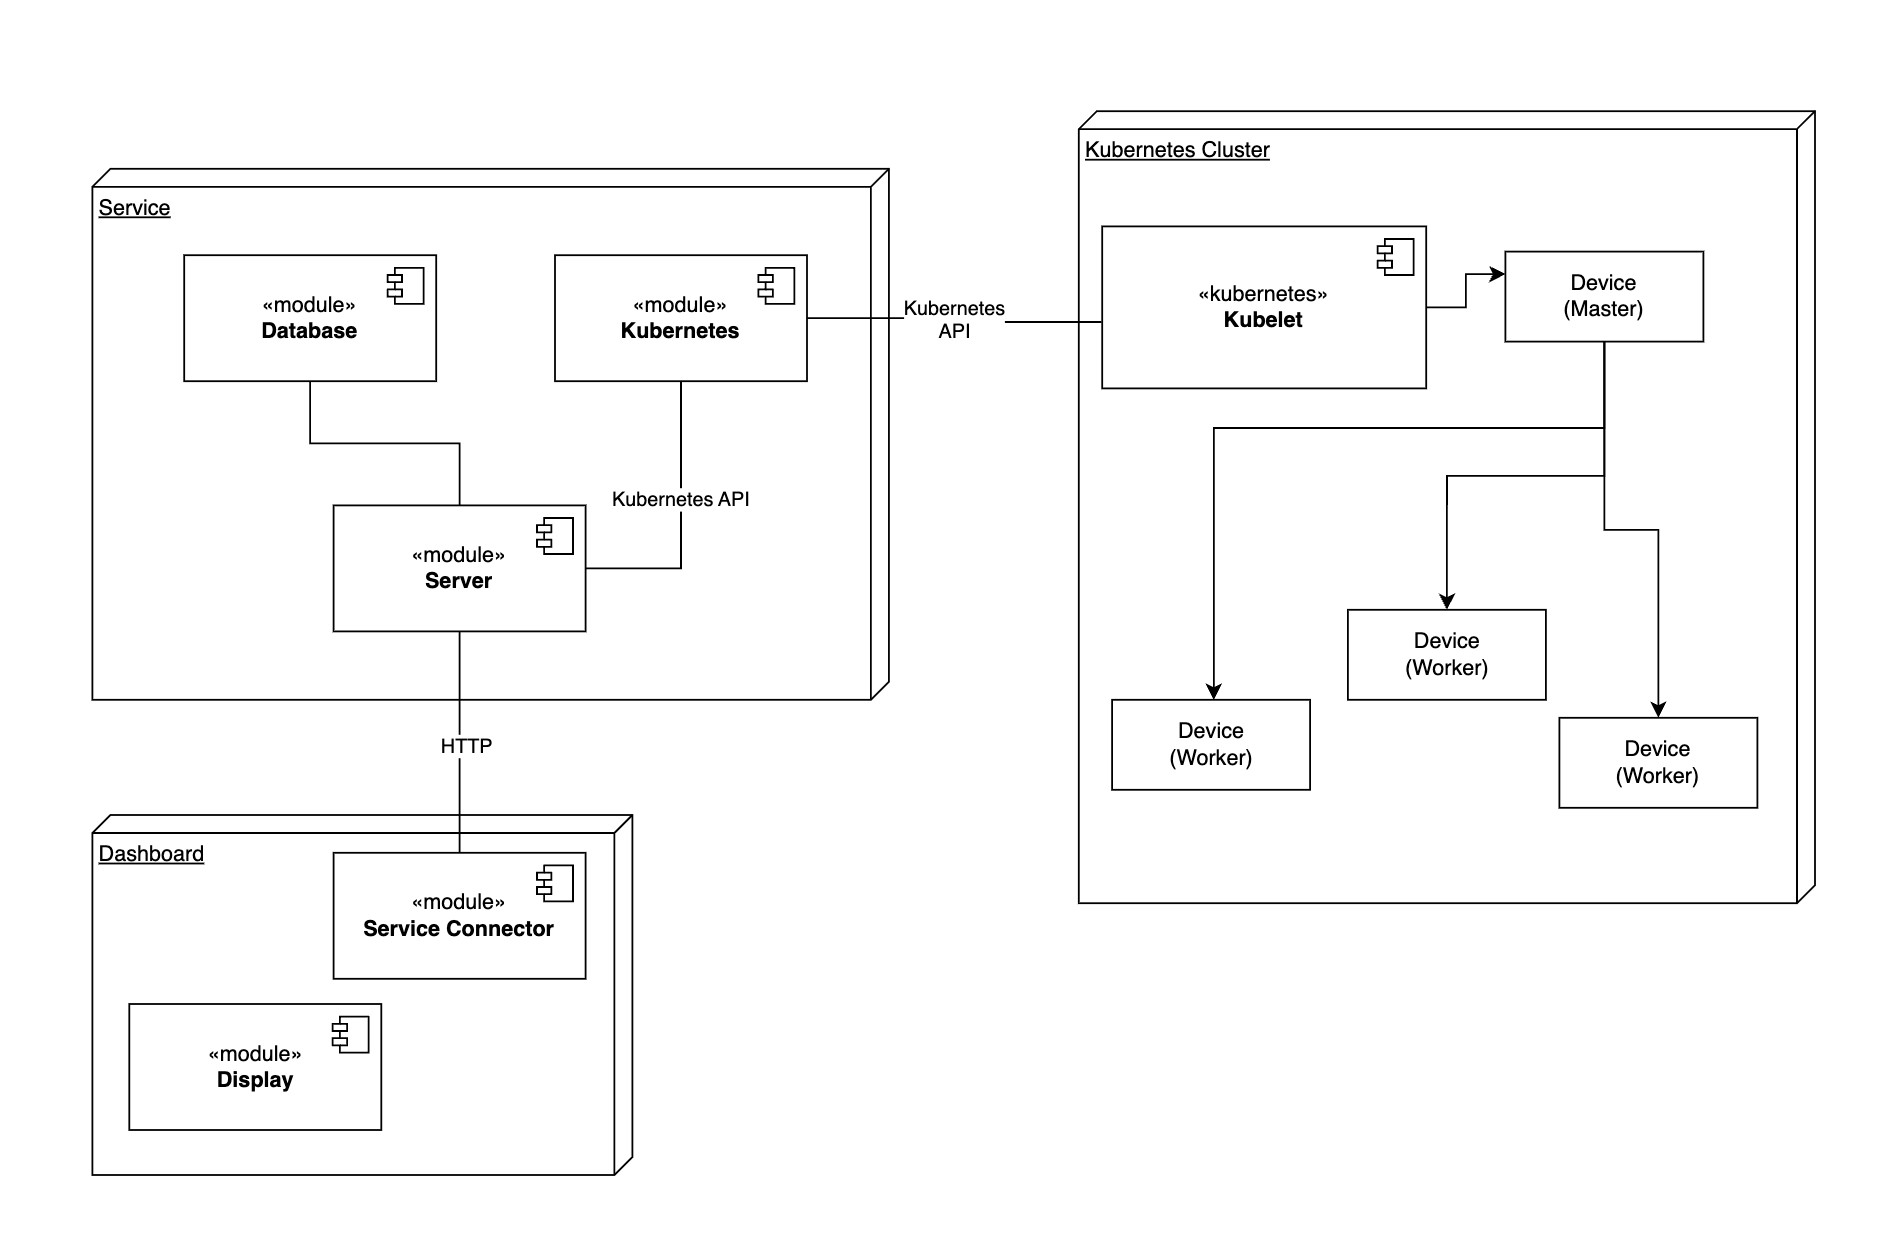
\includegraphics[width=0.9\textwidth]{resources/chapter-3/package-diagram.jpg}
  \caption{Package Diagram}
  \label{fig:package-diagram}
\end{figure}

